\section{Ejercicios}
\begin{enumerate}
\item Un sistema trifásico de secuencia de fases directa y tensión 200 V, alimenta tres impedancias iguales de valor $\overline{Z} = 10\phase {30^\circ}\;\Omega$, conectadas en triángulo. Determinar las corrientes de fase y línea y dibujar el diagrama fasorial.\\
  \emph{Sol.: $\overline{I_{ab}}=20\phase{90^\circ}\;\text{A};\; \overline{I_{bc}}=20\phase{-30^\circ}\;\text{A};\; \overline{I_{ca}}=20\phase{-150^\circ}\;\text{A};$\\
    $\overline{I_{a}}=
    {20\sqrt{3}\phase{60^\circ}\text{A}};\;\overline{I_{b}}={20\sqrt{2}\phase{-60^\circ}\text{A}};\;
    \overline{I_{c}}= {20\sqrt{3}\phase{180^\circ}\text{A}}$}
\item Un sistema trifásico de secuencia de fases inversa y tensión 200
  $\sqrt{3}$ V, alimenta a tres impedancias iguales de valor
  $\overline{Z} = 10 \phase{60^\circ} \,\Omega$, conectadas en
  estrella. Determinar la corriente de línea y el diagrama
  fasorial.\\
  \emph{Sol.:
    $\overline{I_{a}}={20\phase{-150^\circ}\;\text{A}};
    \overline{I_{b}}={20\phase{-30^\circ}\;\text{A}};\;\overline{I_{c}}={20\phase{90^\circ}\;\text{A}}$}
\item Un sistema trifásico de cuatro conductores, de secuencia de
  fases directa y 200$\sqrt{3}$ V, alimenta a tres impedancias:
  $\overline{Z_A} = 10 \phase{60^\circ}\;\Omega$,
  $\overline{Z_B} = 10 \phase{0^\circ}\;\Omega$ y
  $\overline{Z_C} = 10 \phase{-30^\circ}\;\Omega$. Determinar las
  corrientes de línea y
  dibujar el diagrama fasorial.\\
  \emph{Sol.:
    $ \overline{I_{a}}={20\phase{30^\circ}\;\text{A}};\;
    \overline{I_{b}}={20\phase{-30^\circ}\;\text{A}};\;
    \overline{I_{c}}={20\phase{180^\circ}\;\text{A}};\;
    \overline{I_{N}}=14.64\phase{0^\circ}\;\text{A}$}
\item En el sistema trifásico de la Figura~\ref{fig.ejercicio4_BT3} de
  secuencia de fases directa y $f=60$ Hz, el receptor equilibrado
  disipa una potencia total $P_T =51984$ W con un factor de potencia
  de 0,6 en retraso. Sabiendo que el amperímetro indica 76$\sqrt{3}$
  A, determinar:
  \begin{itemize}
  \item Lecturas de los vatímetros 1 y 2
  \item Valor de la impedancia $\overline{Z}$ en forma compleja
  \item Capacidad mínima para mejorar el factor de potencia a 0,95
  \end{itemize}
  \begin{figure}[H]
    \centering
    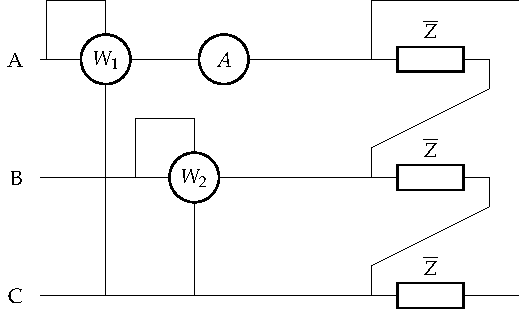
\includegraphics[width=0.5\linewidth]{../figs/ej4_BT3.pdf}
    \caption{Ejercicio 4}
    \label{fig.ejercicio4_BT3}
  \end{figure}
  \emph{Sol.:
    $ W_1=46000.65\,W;\; W_2=5983.35\,W;\;
    \overline{Z}=3+\mathrm{j}\,4\;\Omega;\; C_D=51.31\;mF/fase$}
\item En el sistema trifásico de la Figura~\ref{fig.ej5_BT3}, de
  secuencia de fases inversa y tensión de línea 200$\sqrt{3}$ V, los
  dos receptores son equilibrados, con impedancias
  $\overline{Z_1} = 6+\mathrm{j}8\;\Omega$ y
  $\overline{Z_2} = 8+\mathrm{j}6\;\Omega$. Determinar:
  \begin{itemize}
  \item Lecturas de los amperímetros.
  \item Lecturas de los vatímetros y la potencia compleja total.
  \end{itemize}
  \begin{figure}[H]
    \centering
    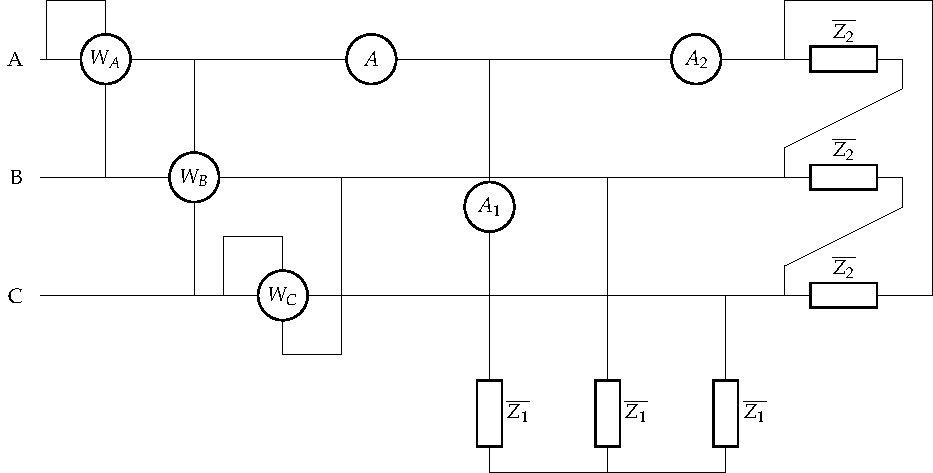
\includegraphics[width=0.9\linewidth]{../figs/ej5_BT3.pdf}
    \caption{Ejercicio 5}
    \label{fig.ej5_BT3}
  \end{figure}
  \emph{Sol.:
    $A=79.40\,A;\;A_1=20\,A;\;A_2=60\,A;\; W_A={27007.43\;\text{W}};\;
    W_B={18013.85\;\text{W}};\;W_C={8993.58\;\text{W}};\;
    \overline{S_T}=36000+\mathrm{j}31200\,VA $}
\item El receptor trifásico de la Figura~\ref{fig.ej6_BT3} tiene
  secuencia de fases inversa y tensión de línea 200$\sqrt{3}$ V. Su
  potencia activa es 12 kW y el vatímetro 2 ($W_2$) indica 6
  kW. Hallar:
  \begin{itemize}
  \item Valor de la impedancia $\overline{Z}$, en forma compleja.
  \item Fasores correspondientes a las intensidades de línea.
  \end{itemize}
  \begin{figure}[H]
    \centering
    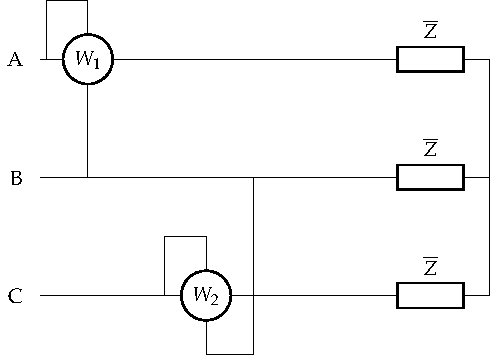
\includegraphics[width=0.4\linewidth]{../figs/ej6_BT3.pdf}
    \caption{Ejercicio 6}
    \label{fig.ej6_BT3}
  \end{figure}
  \emph{Sol.:
    $\overline{Z}=10\phase{0^\circ}\Omega;\;
    \overline{I_a}={20\phase{-90^\circ}\;\text{A}};
    \overline{I_b}={20\phase{30^\circ}\;\text{A}};
    \overline{I_c}={20\phase{150^\circ}\;\text{A}}$}

\item El sistema trifásico de la Figura~\ref{fig.ej7_BT3} es de 380 V
  a 50 Hz y secuencia de fases inversa. $\overline{Z}$ es un elemento
  pasivo ideal, tal que el factor global de potencia es la unidad. El
  motor es de 1,8 CV, rendimiento 90\% y factor de potencia
  0,8. Determinar:
  \begin{itemize}
  \item Impedancia $\overline{Z}$ en forma compleja.
  \item Intensidad en el motor.
  \item Fasores intensidad de línea.
  \item Lectura de los aparatos de medida: V, A, W$_1$, W$_2$ y W$_3$.
  \end{itemize}
  \begin{figure}[H]
    \centering
    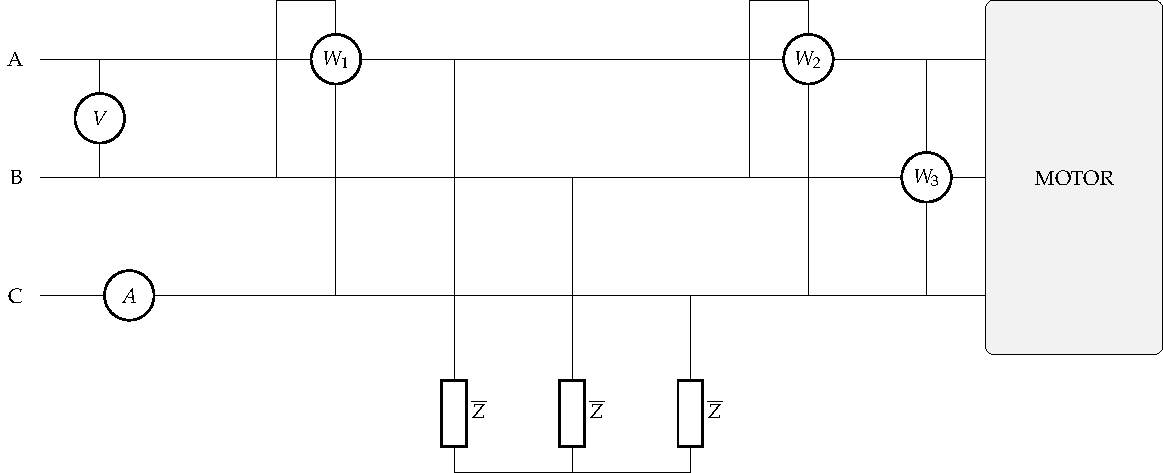
\includegraphics[width=0.9\linewidth]{../figs/ej7_BT3.pdf}
    \caption{Ejercicio 7}
    \label{fig.ej7_BT3}
  \end{figure}

  \emph{Sol.:
    $\overline{Z}={-\mathrm{j}\,129.76}\;\Omega\text{/fase};\;
    I_M=2.83\,A;\;\overline{I_{a}}={2.27\phase{-90^\circ}\;\text{A}};\;
    \overline{I_{b}}={2.27\phase{30^\circ}\;\text{A}};\;
    \overline{I_{c}}={2.27\phase{150^\circ}\;\text{A}};\; W_1=0;\;
    W_2=-645.24W;\; W_3=645.24W$}

\item Una plantación agrícola emplea dos bombas sumergibles para
  extraer agua de un pozo y transportarla a través de un sistema de
  riego por goteo. Estas dos bombas están alimentadas a {400}{V} por
  una línea trifásica en secuencia de fases directa y frecuencia
  ${50}{Hz}$. Una de las bombas funciona con un motor trifásico de
  ${30}{kW}$ y factor de potencia de $0.78$. La otra bomba trabaja con
  un motor de ${7.5}{kW}$ y factor de potencia de $0.67$. La línea que
  alimenta estas dos bombas es resistiva, con resistividad $\rho$ =
  {0.017}{$\Omega$ mm$^2$/m}, longitud de {300}{m} y una sección de
  {35}{mm$^2$}.
  \begin{itemize}
  \item Calcular el triángulo de potencias (potencia activa, reactiva,
    y aparente) de cada carga, y total de las cargas (a la salida de
    la línea).
  \item Calcular el {valor eficaz} de la corriente de línea de cada
    carga, y total.
  \item Determinar la lectura de los siguientes aparatos de medida
    conectados a la entrada de las cargas:
    \begin{itemize}
    \item Un vatímetro en la fase A, midiendo tensión entre las fases
      A y C.
    \item Un vatímetro en la fase B, midiendo tensión entre las fases
      B y C.
    \item Un vatímetro en la fase C, midiendo tensión entre las fases
      B y A.
    \end{itemize}
  \item Calcular el triángulo de potencias a la entrada de la línea.
  \item Calcular el {valor eficaz} de la tensión a la entrada de la
    línea.
  \item Calcular los condensadores que se deben conectar a la salida
    de la línea para mejorar el factor de potencia del sistema hasta
    la unidad, indicando el modo de conexión.  Una vez conectados los
    condensadores del último apartado:
    \begin{itemize}
    \item Calcular el {valor eficaz} de la corriente de línea total.
    \item Calcular el triángulo de potencias a la entrada de la línea.
    \item Calcular el {valor eficaz} de la tensión a la entrada de la
      línea.
    \item Determinar la lectura de los vatímetros descritos
      anteriormente.
    \end{itemize}
  \end{itemize}
  \emph{Sol.:
    $P_1 = {30}{kW};\; Q_1 = {24.07}{kVAr};\; S_1={38.46}{kVA};\; P_2
    = {7.5}{kW};\; Q_2 = {8.31}{kVAr};\; S_2 ={11.19}{kVA}; P_T=
    {37.5}{kW}; \;Q_T= {32.38}{kVAr};\; S_T = {49.55}{kVA};\; I_1 =
    {55.51}{A};\; I_2 = {16.15}{A};\; I_T= {71.52}{A};\; W_{A,AC} =
    {28.10}{kW}; \; W_{B,BC} = {9.40}{kW};\;W_{C, BA} =-
    {18.69}{kW};\; P_g = {39.74}{kW};\; Q_g= {32.38}{kVAr};\; S_g =
    {51.26}{kVA};\;U_g = {413.81}{V};\; C = {214.7}{\mu F/fase};\;
    I_T' = {54.13}{A};\; P_g' = {38.78}{kW};\; Q_g' = {0}{VAr};\; S_g'
    ={38.78}{kVA};\; U' = {413.66}{V};\; W_{A,AC}' = {18.75}{kW};\;
    W_{B,BC}' = {18.75}{kW};\; W'_{C,BA} = {0}{W}$ }
 
\item El circuito de la Figura~\ref{fig.ej9_BT3} es de secuencia de
  fases directa y 50 Hz. Determinar:
  \begin{itemize}
  \item Potencias activas y reactivas totales.
  \item Capacidad mínima de los condensadores a instalar para mejorar
    el factor de potencia total hasta la unidad.
  \item Intensidades de línea, en forma fasorial, una vez mejorado el
    factor de potencia.
  \end{itemize}
  Datos:
  $\overline{Z}_1 = {100\phase{{60}^\circ}}{\Omega};\; W_1 =
  {300}{W};\; W_2 = {300}{W};\; V= {\sqrt{3} \cdot 200}{V}$
  \begin{figure}[H]
    \centering
    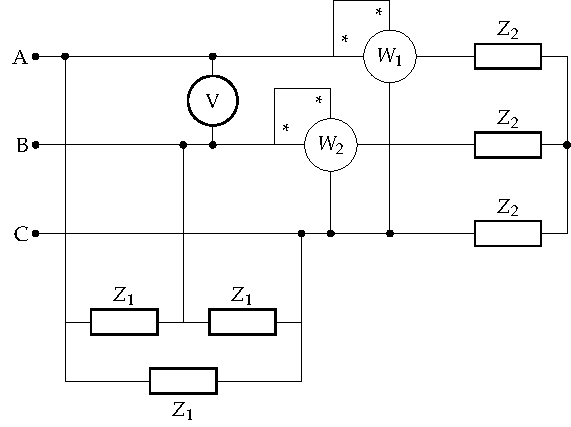
\includegraphics[width=0.5\linewidth]{../figs/ej9_BT3.pdf}
    \caption{Ejercicio 9}
    \label{fig.ej9_BT3}
  \end{figure}
  \emph{Sol.:
    $P_T = {2400} W;\; Q_T =1800\sqrt{3}{VAr};\; C=27.57\,\mu
    F;\;\overline{I}_A = {4\phase{{90^\circ}}}{A}; \;
    \overline{I}_B={4\phase{{-30^\circ}}}{A};\; \overline{I}_C
    ={4\phase{{-150^\circ}}}{A}$}

\end{enumerate}
